\chapter{Lecture 2: Topics in String Theory}

This lecture begins with a deliberate reset. Before discussing the quantum mechanics of black holes, Leonard Susskind returns to the special theory of relativity and rebuilds the geometric idea of a metric from the ground up. The first payoff is operational: light rays are identified by the condition of zero proper time. Only after that rule is firmly in place does the lecture introduce the Schwarzschild metric, distinguish the horizon from the singularity, and then pivot toward the information problem, entropy, and Bekenstein's argument that black-hole entropy is proportional to area. These notes follow Leonard Susskind's lecture closely, with notation normalized where necessary for clarity, and are curated by LazyingArt LLC (\texttt{https://lazying.art}).

\section{Flat Spacetime, Proper Time, and Null Trajectories}

Susskind begins with the simplest setting: neighboring events in flat spacetime. If two infinitesimally separated events differ by \(dt,dx,dy,dz\), then the proper time between them is defined by
\begin{equation}
d\tau^2 = dt^2 - \frac{1}{c^2}\left(dx^2+dy^2+dz^2\right).
\end{equation}
This is the spacetime interval appropriate to special relativity. It is not the Euclidean distance in four dimensions; the spatial pieces enter with the opposite sign.

The lecture immediately turns this definition into a rule for light. If a light ray moves only along the \(x\)-direction, then \(dy=dz=0\), and the condition for the light ray is
\begin{equation}
d\tau^2=0.
\end{equation}
This single equation already contains the statement that light moves with speed \(c\). Indeed,
\begin{align}
0 &= dt^2 - \frac{1}{c^2}dx^2,\\
c^2dt^2 &= dx^2,\\
c\,dt &= \pm dx,
\end{align}
so that
\begin{equation}
\frac{dx}{dt}=\pm c.
\end{equation}
The two signs correspond to left-moving and right-moving light rays.

The key lesson is not the numerical value \(c\) itself. The lecture emphasizes the invariant statement: to determine how light moves in any geometry, one imposes the null condition \(d\tau^2=0\).

\section{Metric Tensors and Spherical Coordinates}

General relativity keeps the same logic but changes the geometry. Susskind says that the metric becomes position-dependent and is described by a metric tensor \(G_{\mu\nu}\). We will use the conventional notation \(g_{\mu\nu}\):
\begin{equation}
ds^2 = g_{\mu\nu}\,dx^\mu dx^\nu.
\end{equation}
Repeated indices are summed over, so this compact expression stands for all quadratic combinations of the spacetime coordinate differentials.

The rule for light does not change. In curved spacetime, just as in flat spacetime, light rays are determined by setting the interval to zero:
\begin{equation}
ds^2=0.
\end{equation}
This is the first major continuity in the lecture: the metric changes, but the null-trajectory rule survives unchanged.

Because the black hole to be studied is spherically symmetric, Susskind next rewrites flat space in spherical coordinates. The angular part is compressed into the metric on the unit two-sphere,
\begin{equation}
d\Omega^2 = d\theta^2 + \sin^2\theta\,d\phi^2.
\end{equation}
For a sphere of radius \(r\), the angular piece becomes \(r^2d\Omega^2\). In units with \(c=1\), the flat spacetime metric may then be written as
\begin{equation}
d\tau^2 = dt^2 - \left(dr^2 + r^2 d\Omega^2\right).
\end{equation}
This is the flat reference form against which the black-hole geometry will be compared.

\section{The Schwarzschild Metric as a Deformation of Flat Space}

At this point the lecture declines to solve Einstein's equations and instead writes down the answer. The black hole has mass \(m\), and its Schwarzschild radius is
\begin{equation}
R_s=\frac{2Gm}{c^2}.
\end{equation}
Once \(c=1\) is adopted, this becomes simply \(R_s=2Gm\).

The factor that controls the deformation of flat space is
\begin{equation}
1-\frac{2Gm}{c^2r} = 1-\frac{R_s}{r}.
\end{equation}
Using that factor, the Schwarzschild line element takes the standard form
\begin{equation}
d\tau^2
=
\left(1-\frac{2Gm}{c^2r}\right)dt^2
-
\frac{dr^2}{1-\frac{2Gm}{c^2r}}
-
r^2d\Omega^2.
\end{equation}

\begin{remark}
The lecture frame preserves the structure of the Schwarzschild factor very clearly, but the left edge of the lower line and some handwritten signs are partially obscured. The form written above is the canonical Schwarzschild metric, chosen because it matches the transcript and reduces to the flat spherical metric as \(r\to\infty\).
\end{remark}

Far from the black hole, \(R_s/r\ll 1\), so the coefficient of \(dt^2\) approaches \(1\), the denominator in the radial term approaches \(1\), and the metric reverts to the flat-space spherical form.

\begin{figure}[h]
\centering

\includegraphics[width=0.82\textwidth]{lecture_02_figure_02.png}
\caption{Whiteboard frame in which the flat spherical line element is written above the Schwarzschild deformation. The factor \(1-\frac{2MG}{c^2r}\), the shorthand \(1-\frac{R_s}{r}\), and a small radial sketch are all visible together.}
\end{figure}

\begin{figure}[h]
\centering
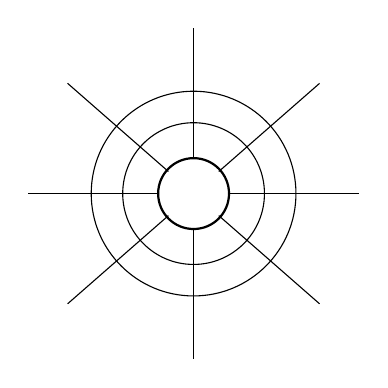
\begin{tikzpicture}[scale=1.0]
\draw[thick] (0,0) circle (0.45);
\draw (0,0) circle (0.9);
\draw (0,0) circle (1.3);
\draw (-2.1,0) -- (-0.45,0);
\draw (0.45,0) -- (2.1,0);
\draw (0,-2.1) -- (0,-0.45);
\draw (0,0.45) -- (0,2.1);
\draw (-1.6,-1.4) -- (-0.32,-0.28);
\draw (0.32,0.28) -- (1.6,1.4);
\draw (-1.6,1.4) -- (-0.32,0.28);
\draw (0.32,-0.28) -- (1.6,-1.4);
\end{tikzpicture}
\caption{A minimal redraw of the radial sketch on the board. It serves only as a schematic cue for spherical symmetry and radial structure.}
\end{figure}

\section{Horizon, Singularity, and the Motion of Radial Light}

From here on the lecture mostly works in units with \(c=1\). Two radii immediately stand out:
\begin{equation}
r=2Gm
\qquad\text{and}\qquad
r=0.
\end{equation}
The lecture insists that these are not the same kind of place. The radius \(r=2Gm\) is the horizon, while \(r=0\) is the singularity. Tidal forces at the horizon are finite, and for a sufficiently large black hole they can be very small. At \(r=0\), by contrast, tidal forces become infinite.

To learn how light behaves, Susskind goes back to the same rule as before: a light ray follows a null trajectory. For a radial light ray, the angles do not change, so
\begin{equation}
d\Omega^2=0.
\end{equation}
The Schwarzschild metric then reduces to
\begin{equation}
0=
\left(1-\frac{2Gm}{r}\right)dt^2
-
\frac{dr^2}{1-\frac{2Gm}{r}}.
\end{equation}
Rearranging gives
\begin{align}
\left(1-\frac{2Gm}{r}\right)dt^2 &= \frac{dr^2}{1-\frac{2Gm}{r}},\\
dr &= \pm\left(1-\frac{2Gm}{r}\right)dt,\\
\frac{dr}{dt} &= \pm\left(1-\frac{2Gm}{r}\right).
\end{align}
The plus sign describes the outgoing branch and the minus sign the ingoing branch.

This is the worked derivation that the lecture wants from the metric. Far from the hole, \(2Gm/r\ll 1\), so the outgoing branch reduces to
\begin{equation}
\frac{dr}{dt}\approx 1,
\end{equation}
exactly as in flat spacetime. Near the horizon,
\begin{equation}
\frac{dr}{dt}\to 0
\qquad\text{as}\qquad
r\to 2Gm.
\end{equation}
In these coordinates, outgoing light rays become slower and slower, and at the horizon they appear to stand still.

\paragraph{A coordinate caveat.}
The lecture pauses over the phrase ``light slows down'' because it can be misleading. The invariant statement is not that light fails to move at the speed of light in some absolute sense. The invariant statement is that light moves on null trajectories. The quantity \(dr/dt\) is a coordinate velocity in Schwarzschild coordinates, and it is this coordinate quantity that tends to zero at the horizon.

\begin{figure}[h]
\centering
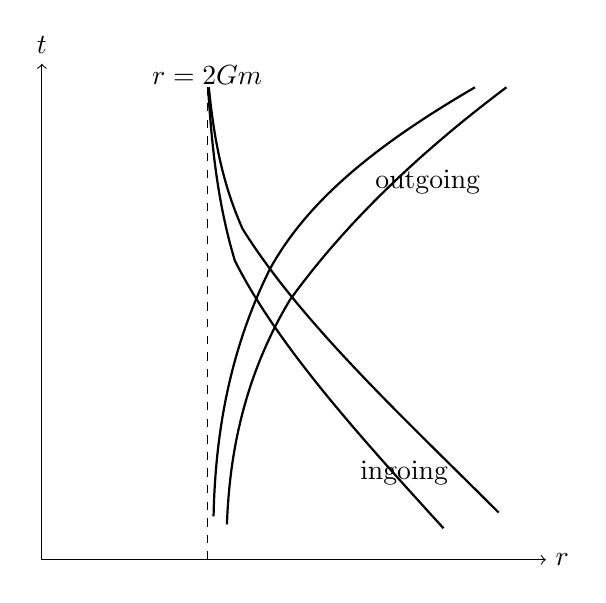
\begin{tikzpicture}[scale=1.0]
\draw[->] (0,0) -- (6.4,0) node[right] {$r$};
\draw[->] (0,0) -- (0,6.3) node[above] {$t$};

\draw[dashed] (2.1,0) -- (2.1,6.0);
\node at (2.1,6.15) {$r=2Gm$};

\draw[thick]
(2.18,0.55) .. controls (2.20,1.5) and (2.35,2.6) .. (2.9,3.7)
.. controls (3.4,4.6) and (4.3,5.3) .. (5.5,6.0);

\draw[thick]
(2.35,0.45) .. controls (2.38,1.3) and (2.55,2.3) .. (3.15,3.3)
.. controls (3.8,4.2) and (4.7,5.1) .. (5.9,6.0);

\draw[thick]
(5.8,0.6) .. controls (4.6,1.8) and (3.3,3.0) .. (2.55,4.2)
.. controls (2.28,4.8) and (2.18,5.4) .. (2.12,6.0);

\draw[thick]
(5.1,0.4) .. controls (4.1,1.5) and (3.0,2.7) .. (2.45,3.8)
.. controls (2.24,4.5) and (2.16,5.2) .. (2.11,6.0);

\node at (4.9,4.8) {outgoing};
\node at (4.6,1.1) {ingoing};
\end{tikzpicture}
\caption{Coordinate-time picture of radial light rays. Outgoing rays become more vertical as they approach the horizon, while ingoing rays asymptotically approach \(r=2Gm\) in coordinate time.}
\end{figure}

The lecture also records the interior moral without yet analyzing the full geometry: once inside the horizon, even light rays aimed outward are carried toward smaller \(r\), and no light signal from inside escapes back out.

\section{From Geometry to the Information Problem}

At this stage Susskind turns sharply from classical geometry to quantum mechanics. From the outside point of view, matter falling toward the black hole gets squeezed closer and closer to the horizon and becomes inaccessible. If nothing ever came back out, that would already be striking, but not yet paradoxical.

The real puzzle begins once one accepts Hawking's claim that black holes radiate. If a black hole emits radiation, then it emits energy; if it emits energy, its mass decreases:
\begin{equation}
E=mc^2.
\end{equation}
Since
\begin{equation}
R_s=\frac{2Gm}{c^2},
\end{equation}
a decrease in \(m\) means a decrease in \(R_s\). A sufficiently long-lived black hole should therefore evaporate away.

The question that now drives the rest of the lecture is immediate: what happens to the information carried by everything that had become trapped, or effectively trapped, at the horizon? Does it disappear? Is it left behind in a remnant? Or does it come out again in the radiation? Before answering that question, Susskind backs up and asks a more elementary one: why should a black hole have entropy at all?

\section{Entropy as Hidden Information}

The lecture chooses a deliberately qualitative route. Information is measured by the number of yes-no questions required to specify a state. A bit is one such yes-no question. In that language, two distinct states remain distinct under time evolution: information does not disappear.

What does happen, in ordinary thermodynamic systems, is that information becomes hidden. Water stirred into a bathtub settles down. The large-scale configuration looks simple, but the microscopic distinctions have only been transferred into the positions and motions of very many molecules. They have not vanished in principle; they have become inaccessible in practice.

\begin{definition}
In the language of this lecture, entropy is the amount of hidden or inaccessible information: the number of bits that are present in the state but unavailable to the observer.
\end{definition}

Susskind then uses this viewpoint to redefine temperature. If one erases a bit from a computer, one does not destroy information outright; one transfers that bit into the surrounding environment, which heats up slightly. This is the Landauer-style motivation behind the thermodynamic relation used in the lecture.

Writing entropy as \(S\), the lecture's normalization is
\begin{equation}
dE = T\,dS.
\end{equation}
Here \(S\) is measured directly in bits, so \(T\) is being interpreted as the energy cost of hiding one additional bit. The chapter will keep this normalization because it is the one actually used in the argument for black-hole entropy.

\section{Bekenstein's One-Bit Argument and the Area Law}

The lecture now returns to the black hole and asks how much it grows when one adds just one more bit of information. A generic photon is not good enough, because a short-wavelength photon carries many additional bits: its arrival point on the horizon can be localized to high accuracy. To suppress that extra information, one chooses a photon with wavelength as long as possible.

There is, however, a limit. A wavelength much longer than the black hole will not enter efficiently. The lecture therefore works right at the margin:
\begin{equation}
\lambda \sim R_s \sim 2Gm,
\end{equation}
with the understanding that this last relation is being read in the \(c=1\) units used through most of the geometric discussion.

The energy of a photon is estimated from
\begin{equation}
E=cp,
\qquad
p\sim \frac{h}{\lambda},
\qquad
E\sim \frac{ch}{\lambda}.
\end{equation}
Susskind is explicit that factors of \(2\), \(2\pi\), and the distinction between \(h\) and \(\hbar\) are being ignored at this stage. Substituting \(\lambda\sim R_s\) gives the one-bit energy increment
\begin{equation}
\Delta E \sim \frac{ch}{R_s}.
\end{equation}
Since one extra hidden bit costs this much energy, the lecture reads off an order-of-magnitude Hawking temperature,
\begin{equation}
T_H \sim \frac{ch}{Gm},
\end{equation}
again suppressing the numerical factors that are not controlled by this crude estimate.

The same one-bit process can be pushed a little further. Using \(E=mc^2\), the added mass is
\begin{equation}
\Delta m \sim \frac{\Delta E}{c^2} \sim \frac{h}{R_s c}.
\end{equation}
Because \(R_s\propto Gm/c^2\), this implies a radius increment
\begin{equation}
\Delta R_s \sim \frac{G\,\Delta m}{c^2}
\sim
\frac{Gh}{R_s c^3}.
\end{equation}
Now comes the crucial scaling step. Since the horizon area is proportional to \(R_s^2\), one has, up to inessential numerical constants,
\begin{equation}
\Delta A \sim R_s\,\Delta R_s \sim \frac{Gh}{c^3}.
\end{equation}
Thus each extra bit increases the horizon area by a universal Planck-scale amount. Equivalently, one bit occupies about one Planck area on the horizon.

This is the content of Bekenstein's insight:
\begin{equation}
S_{\mathrm{BH}} \propto \frac{A\,c^3}{G\hbar}.
\end{equation}
The lecture then adds the historical refinement. Bekenstein argued correctly for the proportionality, but Hawking fixed the exact coefficient:
\begin{equation}
S_{\mathrm{BH}}=\frac{A\,c^3}{4G\hbar}.
\end{equation}

The final conceptual payoff is subtle and important. The Planck constant appears in the denominator. In the classical limit \(\hbar\to 0\), the entropy would diverge. Quantum mechanics does not create the entropy as a small correction; it prevents the entropy from being infinite by quantizing the information that can be hidden at fixed energy.

\section{Summary}

The lecture has a very tight arc. It begins with proper time in flat spacetime and the null condition for light, carries that same diagnostic rule into curved spacetime, and then applies it to the Schwarzschild geometry to isolate the horizon and the singularity. With the horizon picture in place, the discussion turns to hidden information, the thermodynamic relation \(dE=T\,dS\), and finally to Bekenstein's one-bit argument, which leads to the conclusion that black-hole entropy scales with horizon area rather than volume.

Two lessons stand out. First, the invariant statement about light is always geometric: light follows null trajectories. Second, once quantum mechanics is admitted, a black hole is not a dead classical object but a thermodynamic system with a finite entropy,
\[
S_{\mathrm{BH}}=\frac{A\,c^3}{4G\hbar},
\]
and the horizon becomes the natural place where that information is counted.